\documentclass{article}
\usepackage{blindtext}
\usepackage{graphicx} 
\usepackage{tikz}
\usetikzlibrary{trees}
\usepackage{minted}
\usepackage{xcolor}
\usepackage{amsmath}
\usepackage{geometry}
\usepackage[table]{xcolor}
\usepackage{tabularx}
\usepackage{amssymb}
\usepackage{booktabs}

% --- CONTATORI CUSTOM ---
\newcounter{FRnum}
\newcounter{NFRnum}
\newcounter{OBnum}

% \subsubsection* = nessun numero automatico nel testo
% \addcontentsline = aggiunge manualmente la voce al TOC con testo esatto
\newcommand{\frsubsub}[1]{%
  \stepcounter{FRnum}%
  \addcontentsline{toc}{subsubsection}{FR \arabic{FRnum} - #1}%
  \subsubsection*{FR \arabic{FRnum} - #1}%
}

\newcommand{\nfrsubsub}[1]{%
  \stepcounter{NFRnum}%
  \addcontentsline{toc}{subsubsection}{NFR \arabic{NFRnum} - #1}%
  \subsubsection*{NFR \arabic{NFRnum} - #1}%
}

\newcommand{\obsub}[1]{%
  \stepcounter{OBnum}%
  \addcontentsline{toc}{subsubsection}{OB \arabic{OBnum} - #1}%
  \subsection*{OB \arabic{OBnum} - #1}%
}

% --- COLORI ---
\definecolor{headerColor}{HTML}{f2efc2}

% --- HYPERREF (sempre per ultimo) ---
\usepackage[colorlinks=true, linkcolor=gray, urlcolor=gray, citecolor=gray, filecolor=gray]{hyperref}
\usepackage{fancyhdr}
\pagestyle{fancy}

% Pulisce tutti i campi predefiniti
\fancyhf{} 

% Imposta l'altezza dell'intestazione (consigliato per evitare warning)
\setlength{\headheight}{14.5pt}

% Intestazione a sinistra (L)
% Per andare a capo all'interno dell'header, usa \\
\fancyhead[L]{104 - Team Not Found \\ version 1.0} 

% Piè di pagina al centro (C)
\fancyfoot[C]{\thepage} 

% Spessore della linea orizzontale sotto l'header
\renewcommand{\headrulewidth}{0.4pt}
\usepackage{fancyhdr}
\pagestyle{fancy}
\fancyhf{} % Clear all default headers and footers
\fancyhead[R]{104 - Team Not Found \\ version 1.0}\fancyfoot[C]{\thepage} % Center footer with page number
\renewcommand{\headrulewidth}{0.4pt} % Optional: adds a horizontal line under the header 
\begin{document}

\begin{titlepage}
    \centering % Centra gli elementi principali
    {\Huge\bfseries Design of the software \par}
    \vspace{0.5cm}
    {\Large\itshape the definition of the project, the target and the requirements \par}
    \vspace{2cm}
    
    \begin{figure}[h]
        \centering
        
\includegraphics[width=1.0\textwidth]{104okok.png}
    \end{figure}
    
    \vfill

    % Nome del team centrato e molto grande
    {\Huge \textbf{104 - Team Not Found}} \\
    \vspace{0.55cm}

    \begin{flushright}
        
    
        {\large \textbf{Matteo Golinelli, Caterina Alessi, Robin Bertolini, Virginia Ancora}} \\
        \vspace{0.1cm}
        {\large \textit{ \today}}
    \end{flushright}
\end{titlepage}

\cleardoublepage
\phantomsection
\addcontentsline{toc}{section}{Table of Contents}
\tableofcontents

\newpage

% =============================================================================
\section{Context description}
% =============================================================================

\subsection{Purpose of the document}

This document provides an analysis of the application requirements for the Train project.
It is written in plain language and serves as the primary reference for all what concerns the design, development and validation activities for the Deliverable 1.\\

The purpose of this document is to:
\begin{itemize}
    \item present the project context background;
    \item define the project objectives, together with the limitations of our implementation of the project;
    \item identify, describe and provide services to all relevant stakeholders;
    \item define the functional requirements (FR) of the Application System;
    \item define the non-functional requirements (NFR) of the Application System, categorized by quality attribute.
\end{itemize}
The document is written for internal and external users, including our software development team, the Railway-Administration staff, and any external assessors evaluating the completeness and quality of the requirements specification.
\newpage
\section{Project Objectives}

The Project Idea originates from the need of many student and train-travelers to improve, modernize, extend already existing Train Application (like "TrenItalia") to better manage the ticket purchase and management of both route ticket and regional subscription (like the TrentinoTrasporti's one) \\
The solution that we have chosen consists in the development of a web-based software  that consolidates ticketing, journey planning, real-time information, and analytics into a single and complete web-app.\\
The Web Application is designed to serve two primary actor groups:
\begin{itemize}
    \item Customers 
    \subitem - Passengers (only registered)
    \subitem - User of the Web-App (both registered and anonymous)
    \item Train Inspectors
\end{itemize}
Specifically, the Web Application will present all the objectives mentioned below.

\obsub{User-Friendly Interface}
\label{OBJ1}
Provide a user-friendly interface for buying, and managing train tickets, and regional or single-route subscriptions passes, modifying existing bookings, and view any their active subscription at any time.\\
It does not cover the issue of physical tickets, physical ticket printing management.

\obsub{Delay prediction}
\label{OBJ2}
Support journey  planning and optimization through intelligent search filters and delay prediction. The Web-App shall allow passengers to search for links, select preferred travel options, and receive prediction of delays before booking the travel, in order to simplify the organization of other journey or exchanges with other means of transportation.\\
It does not cover the guaranty of real arrival times prediction.

\obsub{Additional Travel-Related booking}
\label{OBJ3}
Allow passengers to book additional travel-related services, including on-board luggage storage, and dedicated bike wagon spaces for bikes and e-bikes.\\
It does not cover the actual operational aspects; it handles only the reservation, not the actual assignment of the actual assigned numbered place reserved.

\obsub{Real-Time Train Information}
\label{OBJ4}
Provide real-time train information, including live occupancy conditions of the wagons and departure/arrival boards, enabling passengers to make informed decisions before their journey.\\
It does not cover historical occupancy analytics or predictive crowding forecasts other than the real-time feed provided by the ticket inspector, which will mark the seats as busy when he validates the ticket/subscription.


\obsub{Track Travel-History}
\label{OBJ5}
Allow registered passengers to track their travel history and participate in some internal loyalty programs, accumulating and viewing loyalty points, linked to their past journeys, with the possibility of converting them into discounts or small gifts.\\
It does not address integration with external loyalty ecosystems other than those that are in our Web-App.

\obsub{Ticket Validation}
\label{OBJ6}
Equip train-inspectors with tools to validate passenger tickets and subscriptions, and to monitor real-time wagon occupancy during service.\\
It does not cover automated gate validation hardware integration or penalty fee management. It does not cover the tap-and-go option of ticket payment.
\obsub{Customer-Support and Refunding }
\label{OBJ7}
Provide the service for the customers to contact the support and ask for information, report something that went wrong and ask for refunding .\\
It does not cover the possibility of changing a  ticket, after the established time defined by internal rules.
\obsub{Shift Schedule for Ticket Inspectors}
\label{OBJ8}
Equip Train Inspectors with the shift schedule to know which train they have to work on everyday.\\
It does not cover the implementation of the possibility of expressing preferences on the place where you work daily.

\obsub{Statistic and Insights for administrative staff}
\label{OBJ9}
Equip Railway Managers with a set of tools to visualize and analyze data and statistics about the train company.\\
It does not develop any type of prediction or action-driven suggestion for future financial actions to be done by the Railway Managers.

\newpage
% =============================================================================
\section{Stakeholders}
% =============================================================================

A stakeholder is anyone or anything that cares about the project or is affected by it. They are essential for shaping the software requirements because their needs tell us what features to build and who we are building them for.
It is also worth noting that a stakeholder is not always a direct user of the application. While some will interact directly with it, others might never touch the software itself but are still heavily affected by its outcomes.

\begin{figure}[htbp] % h=here, t=top, b=bottom, p=page
\begin{center}
\begin{center}
% \resizebox scales the diagram to perfectly fit the width of your page's text area
\resizebox{\textwidth}{!}{%
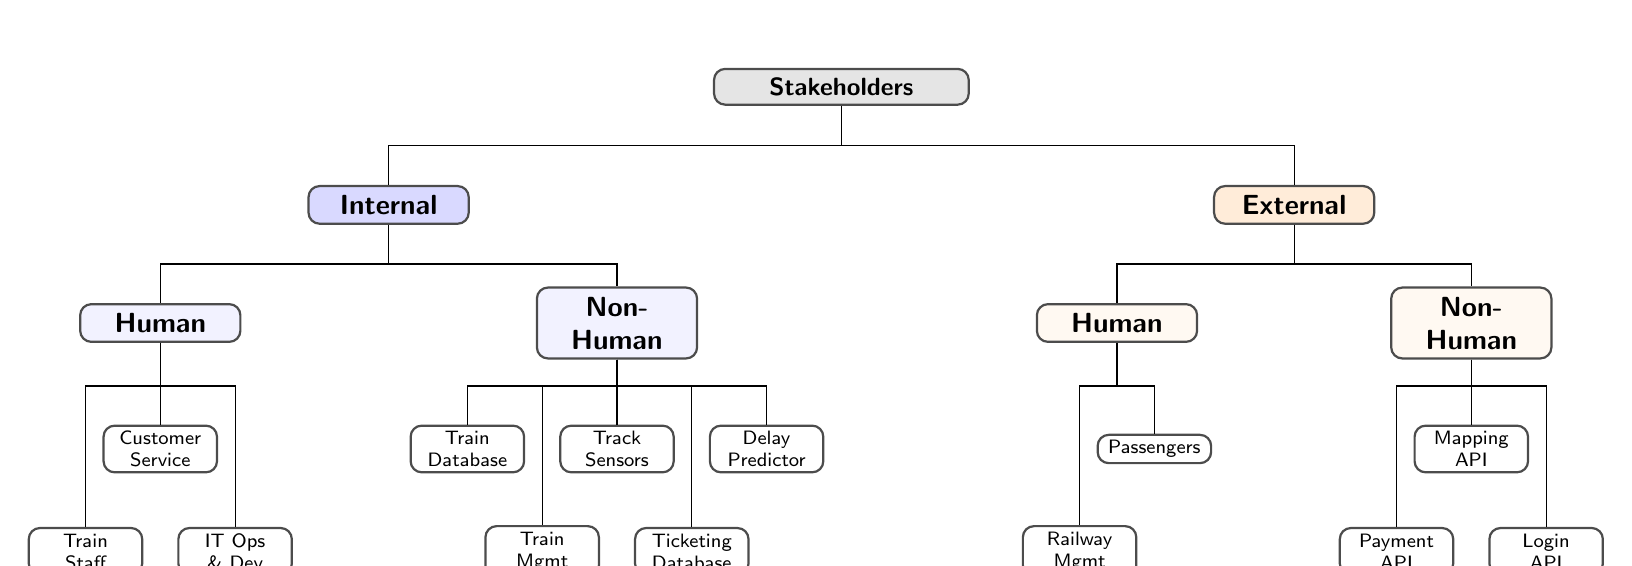
\begin{tikzpicture}[
  edge from parent fork down,
  grow=down,
  % Global box styling
  every node/.style={draw=black!70, thick, rounded corners, fill=gray!10, font=\sffamily\scriptsize, align=center},
  % Level vertical spacing
  level 1/.style={level distance=1.5cm},
  level 2/.style={level distance=1.5cm},
  level 3/.style={sibling distance=0.95cm, level distance=1.6cm},
  % Specific styles
  root/.style={fill=gray!20, font=\sffamily\bfseries\small, text width=3cm},
  internal/.style={fill=blue!15, font=\sffamily\bfseries, text width=1.8cm},
  external/.style={fill=orange!15, font=\sffamily\bfseries, text width=1.8cm},
  leaf/.style={fill=white, text width=1.3cm, inner sep=2pt},
  lowleaf/.style={fill=white, text width=1.3cm, inner sep=2pt, yshift=-1.3cm}
]

\node[root] {Stakeholders}
  % Wide gap to separate the massive Internal and External trees
  child[sibling distance=11.5cm] {node[internal] {Internal}
    % Custom gap for Internal's children
    child[sibling distance=5.8cm] {node[internal, fill=blue!5] {Human}
      child {node[lowleaf] {Train\\Staff}}
      child {node[leaf] {Customer\\Service}}
      child {node[lowleaf] {IT Ops\\\& Dev}}
    }
    child[sibling distance=5.8cm] {node[internal, fill=blue!5] {Non-Human}
      child {node[leaf] {Train\\Database}}
      child {node[lowleaf] {Train\\Mgmt}}
      child {node[leaf] {Track\\Sensors}}
      child {node[lowleaf] {Ticketing\\Database}}
      child {node[leaf] {Delay\\Predictor}}
    }
  }
  child[sibling distance=11.5cm] {node[external] {External}
    % Custom gap for External's children (smaller because there are fewer boxes)
    child[sibling distance=4.5cm] {node[external, fill=orange!5] {Human}
      child {node[lowleaf] {Railway\\Mgmt}}
      child {node[leaf] {Passengers}}
    }
    child[sibling distance=4.5cm] {node[external, fill=orange!5] {Non-Human}
      child {node[lowleaf] {Payment\\API}}
      child {node[leaf] {Mapping\\API}}
      child {node[lowleaf] {Login\\API}}
    }
  };

\end{tikzpicture}%
}
\end{center}
\end{center}
\caption{Stakeholder graph}
\end{figure}

\subsection{INTERNAL}
Inside the organization or development team. Directly involved in building or governing the system.

\subsubsection*{- Human}
People who interact directly or indirectly with the system.
\begin{itemize} 
    \item \textbf{Train staff (Ticket inspector)} \label{STK2}, on-the-ground staff. They interact with the system to check passenger tickets, needing real-time updates on availability and platform changes.
    \item \textbf{Customer Service} \label{STK3}, the team that handles customer support and operations. They need access to user profiles to fix ticketing issues, manage subscriptions, and help passengers. 
    \item \textbf{IT operations and development team} \label{STK5}, the technical staff responsible for the long-term health of the software. They are the primary stakeholders for the 'scalability and maintainability' requirements, needing clean code architecture and monitoring tools.
\end{itemize}

\subsubsection*{- Non-human}
Systems, devices, or services that interact with the system technically.
\begin{itemize}
    \item \textbf{Train database} \label{STK7}, the internal system that stores the physical specifications of the fleet. It is divided into the various types of trains (e.g. regional or InterCity), keeping track of maximum spots available, classes. 
    \item \textbf{Train management system} \label{STK8}, the core operational software that handles live traffic control. Our platform must synchronize with it to ensure the 'when a train leaves' data displayed to users matches reality. 
    \item \textbf{Infrastructure sensors and track control} \label{STK9}, IoT devices positioned at stations and throughout the rail network, they feed real-time data into the system. This constant stream of information keeps timetables and departure times in perfect sync. 
    \item \textbf{Ticketing database} \label{STK10}, the internal storage for all purchases. It has to handle a lot of people buying tickets at the same time so it never accidentally double-books a seat or cargo space.
    \item \textbf{Delay prediction} \label{STK11}, an internal module that analyzes historical data and live track conditions to dynamically update timetables and advise users of expected delays during the booking procedure.
\end{itemize}

\subsection{EXTERNAL}
Outside the organization. Affected by or interacting with the system without building it.

\subsubsection*{- Human}
\begin{itemize}
    \item \textbf{Railway administration/management} \label{STK1}, who assigned the project. Their goal is to obtain the maximum efficiency of the platform by ensuring smooth operations and high accessibility. We provide them with a specific interface to visualize sales and reservation statistics, allowing them to easily monitor current trends.
    \item \textbf{Passengers (registered and anonymous users)} \label{STK12}, the main end-users for the commercial side of the app. Their care about convenience and reliability. They use the platform to check timetables, find their platform, and buy tickets. They expect the system to be highly responsive, even during peak hours.
\end{itemize}

\subsubsection*{- Non-human}
\begin{itemize}
    \item \textbf{Payment gateway API}\label{STK16}, an outside service (e.g., Stripe or PayPal) responsible for handling the financial transactions. Because of the requirement for robustness to concurrent accesses (especially during high-traffic purchasing times), our platform heavily depends on this system's reliability.
    \item \textbf{Mapping and routing API}\label{STK17}, an external service for visually rendering the network. It provides the geographical data necessary to display the list of stations and connections to the users planning their trips.
    \item \textbf{Login API}\label{STK18}, an outside service that takes care of handling the login process and users credentials.
\end{itemize}

\newpage
% =============================================================================
\section{Functional requirements}
\label{sec:functional-requirements}
% =============================================================================

\subsection{ANONYMOUS USER MANAGEMENT}
\label{sec:ANONYMOUS USER MANAGEMENT}
\frsubsub{Search train}
\label{FR1}
The user can search for trains by indicating the stations of departure and arrival, the date and time of departure, the type of train, the number and type of passengers, the type of journey (\hyperref[NFR4]{NFR 4}, \hyperref[NFR6]{NFR 6}).

\frsubsub{Select class of travel}
\label{FR2}
In addition to \hyperref[FR1]{FR 1}, the user can select the available class of travel (standard, business).

\frsubsub{Visualization results}
\label{FR3}
The user can see a list of available trains based on the inserted information (\hyperref[FR1]{FR 1}) from which to choose the best solution for him/her.

\frsubsub{Trip details}
\label{FR4}
The user can see the train ID, the intermediate stations, the estimated time of arrival and departure and the track at each of them, the total trip duration, the services of the train (bike transport, disabled people, type of class).

\frsubsub{Intelligent filters to search for trains}
\label{FR5}
Following \hyperref[OBJ2]{OB 2}, the user can ordinate the displayed results (\hyperref[FR3]{FR 3}) based on some specific criteria (like delay prediction, \hyperref[NFR5]{NFR 5}, \hyperref[NFR24]{NFR 24}).

\frsubsub{Departure/Arrival boards}
\label{FR6}
Following \hyperref[OBJ4]{OB 4}, the user can see the departures/arrivals board of the selected station.

\frsubsub{Change language}
\label{FR7}
The user can select the language (\hyperref[NFR22]{NFR 22}) he/she prefers to better understand  the website.

\frsubsub{Seat selection}
\label{FR8}
In addition to \hyperref[FR2]{FR 2}, the user can select the preferred seat through a the train map (\hyperref[NFR24]{NFR 24}).

\frsubsub{Reserve luggage storage}
\label{FR9}
Following \hyperref[OBJ3]{OB 3}, the user can reserve a place for his/her luggage in an apposite area of the train if it is too big to be put over/under the seat.

\frsubsub{Reserve bike wagon}
\label{FR10}
Following \hyperref[OBJ3]{OB 3}, the user can reserve a place for his/her bike in the apposite wagon (if not a folding bike). A bike wagon can contain around 7 bikes.

\frsubsub{Select on the map}
\label{FR11}
In addition to \hyperref[FR1]{FR 1}, the user can instead select the stations of departure and arrival directly on a map (\hyperref[NFR24]{NFR 24}).

\frsubsub{Registration}
\label{FR12}
The user can register providing name, surname, email and a secure password (\hyperref[NFR16]{NFR 16}) and accepting a transparent privacy policy form (\hyperref[NFR23]{NFR 23}, \hyperref[NFR25]{NFR 25}, \hyperref[NFR27]{NFR 27}). 
For ticket inspector, customer service, and admins registration, there will be further verification (specific credentials, \hyperref[FR31]{FR 31},\hyperref[NFR17]{NFR 17}).


\subsection{REGISTERED USER MANAGEMENT}
\label{sec:REGISTERED USER MANAGEMENT}
\frsubsub{Ticket purchase}
\label{FR13}
Following \hyperref[OBJ1]{OB 1}, after searching (\hyperref[FR1]{FR 1}) and selecting the train from the results (\hyperref[FR3]{FR 3}), the registered passenger can buy a ticket (\hyperref[NFR19]{NFR 19}, \hyperref[NFR23]{NFR 23}, \hyperref[NFR24]{NFR 24}).

\frsubsub{Subscription purchase}
\label{FR14}
Following \hyperref[OBJ1]{OB 1}, the registered passenger can purchase a subscription (\hyperref[NFR19]{NFR 19}, \hyperref[NFR23]{NFR 23}, \hyperref[NFR24]{NFR 24}) indicating the stations of departure and arrival, the duration of the subscription, the class of travel (\hyperref[FR2]{FR 2}), the type of train.

\frsubsub{Train status search}
\label{FR15}
Following \hyperref[OBJ4]{OB 4}, the registered user can see its current location by inserting the train ID or the date and time of departure (between two or in which station) with the scheduled and estimated time, in case of delay (\hyperref[OBJ2]{OB 2}), of departure and arrival at each of the previous and following stations (\hyperref[NFR8]{NFR 8}).

\frsubsub{Modify ticket}
\label{FR16}
Following \hyperref[OBJ1]{OB 1}, the registered passenger can change the date and time of departure of an already purchased ticket (\hyperref[FR13]{FR 13}) up to 24 hours before the original departure, after the 24 hours he/she can change only the time (\hyperref[NFR23]{NFR 23}).

\frsubsub{Booking history}
\label{FR17}
Following \hyperref[OBJ5]{OB 5}, the registered passenger can make the search for a train (\hyperref[FR1]{FR 1}) faster using the history of past purchases (departure and arrival stations often selected).

\frsubsub{Active tickets/subscriptions view}
\label{FR18}
Following \hyperref[OBJ1]{OB 1}, the registered user can see purchased tickets/subscriptions (\hyperref[FR13]{FR 13}/\hyperref[FR14]{FR 14}) in an apposite section of the website.

\frsubsub{Loyalty points collection}
\label{FR19}
Following \hyperref[OBJ5]{OB 5}, the registered passenger gains a loyalty point each euro spent (i.e. 14,50 euros equals 14 points).

\frsubsub{Loyalty points balance}
\label{FR20}
Following \hyperref[OBJ5]{OB 5}, the registered passenger and the customer service can see the loyalty points balance (\hyperref[FR19]{FR 19}) in an apposite section of the website.

\frsubsub{Add travel companions}
\label{FR21}
The registered passenger can add other registered (\hyperref[FR12]{FR 12}) users to purchase the ticket/subscription (\hyperref[FR13]{FR 13}/\hyperref[FR14]{FR 14}) also for them.

\frsubsub{Contact customer service}
\label{FR22}
Following \hyperref[OBJ7]{OB 7}, the registered passenger and the inspector can contact the customer service through a form to request partial/full refund.

\frsubsub{Route changes notification}
\label{FR23}
The users are notified in real-time (\hyperref[NFR8]{NFR 8}) in case of changes on the route and consequential delays (\hyperref[NFR23]{NFR 23}).

\frsubsub{Ticket/subscription validation}
\label{FR24}
Following \hyperref[OBJ6]{OB 6}, the inspector can validate the passenger's ticket or subscription on the train.

\frsubsub{Shift schedule display}
\label{FR25}
Following \hyperref[OBJ8]{OB 8}, the inspector and the customer support staff can see their shift schedule on an apposite section of the website.

\frsubsub{Occupancy tracking}
\label{FR26}
Following \hyperref[OBJ4]{OB 4}, the inspector can mark the occupied seats, during validation (\hyperref[FR24]{FR 24}) to provide insights on the capacity of the wagon.

\frsubsub{Account elimination}
\label{FR27}
The registered user can delete his/her account and all the data provided at registration (\hyperref[FR12]{FR 12}, \hyperref[NFR23]{NFR 23}).

\frsubsub{Log-in}
\label{FR28}
The registered user can log-in the website by clicking on an apposite section (\hyperref[NFR20]{NFR 20}, \hyperref[NFR24]{NFR 24}).

\frsubsub{Change Password}
\label{FR29}
The registered user can change his/her password in case he/she forgot or lost it (\hyperref[NFR23]{NFR 23}). 

\frsubsub{Retrieve password}
\label{FR30}
Following \hyperref[OBJ7]{OB 7}, the registered user can recover his/her password to then change it (\hyperref[FR29]{FR 29}) by contacting customer support (\hyperref[FR23]{FR 23}).

\frsubsub{Access to specific area}
\label{FR31}
Following \hyperref[OBJ9]{OB 9}, the registered user (only with provided credentials, \hyperref[NFR17]{NFR 17}) can access an area dedicated to specific actions (like viewing insights for admins, \hyperref[FR32]{FR 32}).

\frsubsub{View insights and statistics}
\label{FR32}
Following \hyperref[OBJ9]{OB 9}, the registered user can view charts and tables to analyze statistics and information of sells, revenue and bookings. 

\frsubsub{Delay Prediction}
\label{FR33}
Following \hyperref[OBJ2]{OB 2}, the registered user can see a delay prediction while booking the itinerary and during the voyage (\hyperref[NFR5]{NFR 5}, \hyperref[NFR8]{NFR 8}, \hyperref[NFR24]{NFR 24}).

\frsubsub{Log-out}
\label{FR34}
The registered user can log out from the website when he finished to use it.
\vspace{2.0em}
\renewcommand{\arraystretch}{1.5}

\begin{figure}[htbp]
\centering
\resizebox{1.0\textwidth}{!}{%
\begin{tabularx}{\textwidth}{>{\bfseries}l X}
\toprule
\rowcolor{headerColor}
User Role & Associated Functional Requirements (FR) \\
\midrule
Anonymous User & 
\hyperref[FR1]{FR 1}, \hyperref[FR2]{FR 2}, \hyperref[FR3]{FR 3}, \hyperref[FR4]{FR 4}, 
\hyperref[FR5]{FR 5}, \hyperref[FR6]{FR 6}, \hyperref[FR7]{FR 7}, 
\hyperref[FR11]{FR 11}, \hyperref[FR12]{FR 12} \\

Registered Passenger &
\hyperref[FR1]{FR 1}, \hyperref[FR2]{FR 2}, \hyperref[FR3]{FR 3}, \hyperref[FR4]{FR 4},
\hyperref[FR5]{FR 5}, \hyperref[FR6]{FR 6}, \hyperref[FR7]{FR 7},
\hyperref[FR8]{FR 8}, \hyperref[FR9]{FR 9}, \hyperref[FR10]{FR 10},
\hyperref[FR11]{FR 11}, \hyperref[FR13]{FR 13}, \hyperref[FR14]{FR 14},
\hyperref[FR15]{FR 15}, \hyperref[FR16]{FR 16}, \hyperref[FR17]{FR 17},
\hyperref[FR18]{FR 18}, \hyperref[FR19]{FR 19}, \hyperref[FR20]{FR 20},
\hyperref[FR21]{FR 21}, \hyperref[FR22]{FR 22},
\hyperref[FR27]{FR 27}, \hyperref[FR28]{FR 28},
\hyperref[FR29]{FR 29}, \hyperref[FR30]{FR 30},
\hyperref[FR33]{FR 33} \\

Ticket Inspector &
\hyperref[FR4]{FR 4}, \hyperref[FR6]{FR 6}, \hyperref[FR7]{FR 7},
\hyperref[FR15]{FR 15}, \hyperref[FR22]{FR 22},
\hyperref[FR23]{FR 23}, \hyperref[FR24]{FR 24},
\hyperref[FR25]{FR 25}, \hyperref[FR26]{FR 26} \\

Customer Service &
\hyperref[FR18]{FR 18}, \hyperref[FR20]{FR 20},
\hyperref[FR23]{FR 23}, \hyperref[FR25]{FR 25} \\

Railway Administration &
\hyperref[FR7]{FR 7}, \hyperref[FR27]{FR 27},
\hyperref[FR28]{FR 28}, \hyperref[FR29]{FR 29},
\hyperref[FR30]{FR 30}, \hyperref[FR31]{FR 31},
\hyperref[FR32]{FR 32} \\

\bottomrule
\end{tabularx}%
}
\caption{Table of Functional Requirements and Actors}
\end{figure}


\newpage
% =============================================================================
\section{Non-functional requirements}
% =============================================================================

\subsection{ORGANIZATIONAL REQUIREMENTS - DEVELOPMENT}

\nfrsubsub{Web-based implementation}
\label{NFR1}
The software has to be a web application that can be accessed by any major operating system (Windows, Linux, MacOs) through a secure and encrypted \textit{https} protocol (satisfy security \hyperref[NFR15]{NFR 15}, \hyperref[NFR16]{NFR 16}).

\nfrsubsub{Cross-browser compatibility}
\label{NFR2}
The web-app will have to be compatible with the main browsers versions: Google Chrome, Mozilla Firefox, Microsoft Edge, and Safari, starting from 2022.

\nfrsubsub{Mobile responsiveness}
\label{NFR3}
The software must be accessible from PC, SMARTPHONE, TABLETS and MOBILES.


\subsection{PRODUCT REQUIREMENTS - IMPLEMENTATION}

\nfrsubsub{Train search}
\label{NFR4}
The software must search trains by:
\begin{itemize}
    \item Type of train: Frecce, Intercity, Regionale
    \item Type of passengers: adult and child
    \item Type of travel: only one way travel or round trip
\end{itemize}
As explained in \hyperref[FR1]{FR 1}

\nfrsubsub{Train filter}
\label{NFR5}
The software must filter trains (after search) by:
\begin{itemize}
    \item Price
    \item Trip time
    \item Probability of delays
    \item Probability of being crowded
\end{itemize}
As explained \hyperref[FR5]{FR 5}

\newpage

\subsection{PRODUCT REQUIREMENTS - PERFORMANCE}

\nfrsubsub{Train search performance}
\label{NFR6}
The software has to address any user-query (\textit{i.e. \hyperref[NFR4]{NFR 4}}) within 1-2 seconds.

\nfrsubsub{Page load time}
\label{NFR7}
The web page load time should be between 2-3 seconds, any other web-page should not take more than 2 seconds to load.

\nfrsubsub{Real-time data updates}
\label{NFR8}
The train position (not precise) should be accessible from user at any time, the system should update every minute \hyperref[FR15]{FR 15}. \textit{ie.: the train is between Bologna and Ravenna at 19:15/ The train has arrived in Parma station at 7:54.}

\nfrsubsub{Concurrent user capacity}
\label{NFR9}
The software has to withstand a synchronous utilization of at least 2 million users (train staff, passengers and un-registered users ecc...).


\subsection{PRODUCT REQUIREMENTS - SCALABILITY}

\nfrsubsub{User scalability}
\label{NFR10}
The software has to be suitable for at least 20 million users (included train staff, passengers, and non-registered users).

\nfrsubsub{Data storage scalability}
\label{NFR11}
Storage has to be large enough and adaptable to \hyperref[NFR10]{NFR 10} and \hyperref[NFR9]{NFR 9}. Moreover a good estimation: 
\begin{itemize}
    \item Users $\rightarrow 60\,\text{GB}$
    \item Tickets (5 years) $\rightarrow 1.8\,\text{TB}$
    \item Real-time train logs (1 year) $\rightarrow 1\,\text{TB}$
    \item Operational logs (3--6 months) $\rightarrow \text{9--36 TB}$
    \item Assets (applications' files) $\rightarrow \text{10--50 GB}$
\end{itemize}

For a total of $\sim \text{12--40 TB}$

\nfrsubsub{Traffic scalability}
\label{NFR12}
Traffic through the servers should be able to withstand \hyperref[NFR9]{NFR 9} and \hyperref[NFR10]{NFR 10} in order to reduce downtime to 1\% monthly. Furthermore with a good approximation: 
\begin{itemize}
    \item Sustained throughput $\rightarrow \text{4--6 GB/s}$
    \item Peak throughput $\rightarrow \text{8--12 GB/s}$
\end{itemize}
With a total annual data transfer of $\sim \text{100–140 PB/year}$ 

\subsection{PRODUCT REQUIREMENTS - RELIABILITY}

\nfrsubsub{System availability}
\label{NFR13}
The system should be accessible from Italy. Moreover, the monthly average up-time should not be less than 99\%.

\nfrsubsub{Data backup}
\label{NFR14}
Data should be backed up every day, stored in some backup storage following the \hyperref[sec:compliance]{PRODUCT REQUIREMENTS - COMPLIANCE} section.

\nfrsubsub{Session timeout}
\label{NFR15}
The time to terminate the inactive log-in user session will have to be no more than 30 minutes so that will allow the \hyperref[sec:security]{PRODUCT REQUIREMENTS - SECURITY}.

\subsection{PRODUCT REQUIREMENTS - SECURITY}
\label{sec:security}

\nfrsubsub{Secure password requirements}
\label{NFR16}
The password should be at least 8 characters long, containing letters and numbers (when registering \hyperref[FR12]{FR 12}) to keep user personal information secure. 

\nfrsubsub{Specific registration/access control}
\label{NFR17}
The access of specific users is restricted by special credentials (\textit{i.e. unique ID}) that are obtained after further verification and evidence approval (\textit{i.e. human}) \hyperref[NFR16]{NFR 16}. The credentials must display a page exclusively for ticket inspectors/admins/customer service, and it should be updated based on load time and up-time. (\hyperref[NFR7]{NFR 7} and \hyperref[FR13]{FR 13}).

\nfrsubsub{Encryption standards}
\label{NFR18}
Users' data should be safely stored in an encrypted database, whose private key is kept offline and in a secure place.

\nfrsubsub{Payment security}
\label{NFR19}
Different payment methods should be implemented, such as the main providers Visa, Mastercard, Google Pay, Apple Pay, and PayPal. Payment security is guaranteed by such third-party agency.

\nfrsubsub{Authentication security}
\label{NFR20}
Each user should be logged in (\hyperref[FR28]{FR 28}) to buy a title or to perform any important action, the log-in page should allow a maximum of 5 failed attempts per minute per IP for each account to prevent brute-force, and security should then be guaranteed by: \hyperref[NFR16]{NFR 16} and \hyperref[NFR17]{NFR 17}.

 \newpage

\subsection{PRODUCT REQUIREMENTS - USABILITY}

\nfrsubsub{User intuitiveness and accessibility}
\label{NFR21}
The software should be easy and straightforward to use, accessible for everyone, even tourists that speak other languages (\hyperref[NFR22]{NFR 22}). The options to choose when booking a train should be clear (\textit{i.e., implementing a map to choose stations of departure and arrival}). In addition, trained personnel must be easily understood of any action taken. At least 90\% \% of the test users have to be able to complete the main tasks (\textit{i.e., registration, login, and main workflow actions}) without external instructions during usability testing. Functional requirements like \hyperref[FR26]{FR 26} and \hyperref[FR15]{FR 15} shall be developed to provide a user-friendly and better  user experience environment.

\nfrsubsub{Multi-language support}
\label{NFR22}
The web-app should be mainly in Italian since we provide a service for North Italy, although English translation should be possible for international users \hyperref[FR7]{FR7}.

\subsection{PRODUCT REQUIREMENTS - REPORTING}
\nfrsubsub{Email notifications}
\label{NFR23}
After a user has performed important actions with their account, any change should be notified via email within 1 minute in order to maintain security level high \textit{(e.g., booked/modified ticket [\hyperref[FR13]{FR13},\hyperref[FR16]{FR16}], changed route [\hyperref[FR23]{FR23}], operation on account [\hyperref[FR12]{FR12}], [\hyperref[FR27]{FR27}]  or changed password [\hyperref[FR29]{FR29}])} for any further clarification any user must contact customer service as explained \hyperref[FR22]{FR 22}.

\subsection{EXTERNAL REQUIREMENTS - COMPATIBILITY}

\nfrsubsub{Login, security, maps and payment APIs and delay prediction}
\label{NFR24}
The system has to handle integration with several external services in order to fulfill several requirements. Delay prediction (\hyperref[STK11]{DELAY PREDICTION}) which must function thanks to an estimation model trained on our data (delays, crowding, most chosen routes, ecc.); maps (\hyperref[STK18]{MAP}), log-in and payment \hyperref[STK18]{Log-in \& PAYMENT} APIs.

\subsection{EXTERNAL REQUIREMENTS - COMPLIANCE}
\label{sec:compliance}

\nfrsubsub{GDPR compliance}
\label{NFR25}
The system must fully be developed according with the General Data Protection Regulation (GDPR) regarding the collection, processing, and storage of personal data for all users: \textit{{\href{https://eur-lex.europa.eu/eli/reg/2016/679/oj}{Regulation (EU) 2016/679}, adopted on April 14, 2016}}.

\nfrsubsub{Data retention policies}
\label{NFR26}
User data and transaction logs must be retained for a period, 3-6 month, after which sensitive personal information must be securely purged or anonymized.

\nfrsubsub{Privacy policy transparency}
\label{NFR27}
The application must supply a evident and easily accessible Privacy Policy that informs users exactly what data is being gathered, how it is used, and how they can exercise their right to be forgotten.

\vspace{2.0em}

\begin{figure}[htbp]
\begin{center}
\resizebox{\textwidth}{!}{%
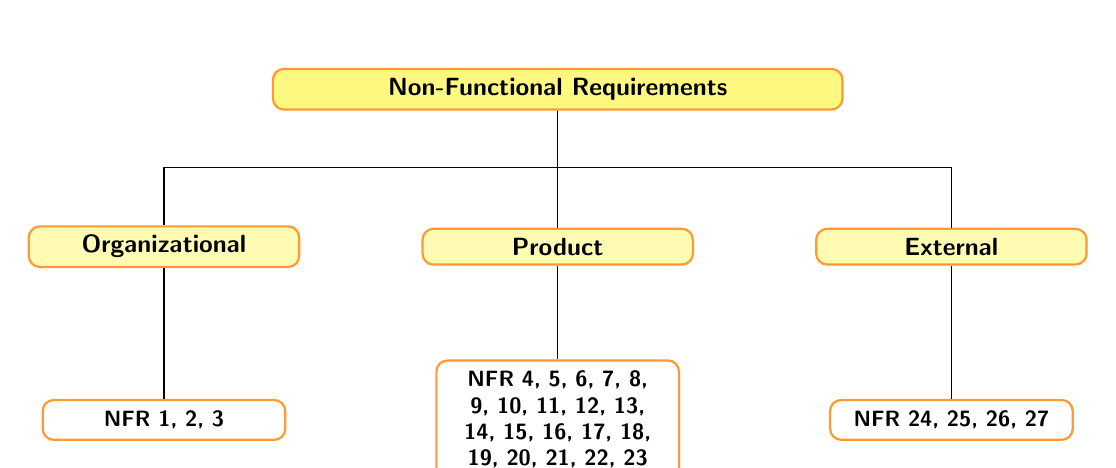
\begin{tikzpicture}[
  edge from parent fork down,
  grow=down,
  every node/.style={draw=orange!80, thick, rounded corners, fill=yellow!10, font=\sffamily\footnotesize, align=center},
  level 1/.style={level distance=2cm, sibling distance=14cm},
  level 2/.style={level distance=2.2cm, sibling distance=6cm},
  level 3/.style={level distance=2cm, sibling distance=3.5cm},
  root/.style={fill=yellow!50, font=\sffamily\bfseries\small, text width=7cm},
  category/.style={fill=yellow!30, font=\sffamily\bfseries\small, text width=3.2cm},
  subcategory/.style={fill=yellow!20, font=\sffamily\bfseries, text width=3cm},
  leaf/.style={fill=white, text width=2.8cm, inner sep=4pt}
]
\node[root] {Non-Functional Requirements}
  child[sibling distance=5cm] {node[category] {Organizational}
    child {node[leaf] {\textbf{NFR 1, 2, 3}}}
  }
  child[sibling distance=14cm] {node[category] {Product}
    child {node[leaf] {\textbf{NFR 4, 5, 6, 7, 8, 9, 10, 11, 12, 13, 14, 15, 16, 17, 18, 19, 20, 21, 22, 23}}}
  }
  child[sibling distance=5cm] {node[category] {External}
    child {node[leaf] {\textbf{NFR 24, 25, 26, 27}}}
  };
\end{tikzpicture}%
}
\end{center}
\caption{Non-functional requirement graph}
\end{figure}

\end{document}